\documentclass[a4paper,12pt]{article}
\usepackage{graphicx}
\usepackage{amsmath, amssymb}
\usepackage{geometry}
\usepackage{booktabs}
\usepackage[colorlinks=true, linkcolor=blue, urlcolor=blue]{hyperref}

\geometry{left=2.5cm,right=2.5cm,top=3cm,bottom=3cm}
\usepackage{float}

\title{Design of a Fully Differential Amplifier Using a Folded Cascode with Gain Boosting}
\author{Or Fachima  \ Arsen Arutyunov }
\date{12/02/2025}

\begin{document}

\maketitle
\begin{abstract}
This report presents the design and implementation of a high-performance fully differential amplifier using BiCMOS8HP technology. The design employs a folded cascode topology with gain boosting, achieving an open-loop gain of 95.8 dB and a gain-bandwidth product of 108.1 MHz. The amplifier demonstrates excellent stability with a phase margin of 88° and a settling time of 41 ns for a 0.3V differential step. A specialized feedback network effectively mitigates noise, achieving a dynamic range of 80.05 dB while maintaining high-speed operation. The design features a high CMRR of 250 dB and operates from a 1.8V supply with a total power consumption of 6.287 mW. These results highlight the amplifier’s suitability for high-precision analog applications.
\end{abstract}



\section{Circuit Topology}
Initially, as presented in our design review, we selected a simple symmetric differential amplifier topology, similar to an OTA but split into two. Over time, we realized that this topology was problematic and would not meet the required specifications for two reasons:

\begin{itemize}
    \item The inherent trade-off between GBW and settling time became a significant limitation. Attempts to improve settling time by increasing gain resulted in reduced bandwidth and slower overall response.
    
    \item Being a two-stage amplifier, achieving the required GBW while maintaining adequate phase margin proved challenging. The additional pole from the second stage complicated frequency compensation, making it difficult to optimize for both speed and stability.
\end{itemize}

To overcome these limitations, we switched to a folded cascode topology - a single-stage design that naturally provides better frequency response characteristics. However, initial testing revealed that while this topology offered improved speed, we couldn't achieve sufficient DC gain for our requirements. This led us to implement gain-boosting stages, which allowed us to significantly enhance the DC gain while preserving the excellent frequency response characteristics of the folded cascode structure.
\subsection{Main Circuit Schematic}
Figure \ref{fig:main_circuit} shows the schematic of the main amplifier circuit. The folded cascode structure is employed to maximize gain while maintaining stability. The circuit consists of a differential input stage, a folded cascode gain stage, and a common-mode feedback (CMFB) circuit to regulate the output common-mode voltage.

\begin{figure}[h]
    \centering
    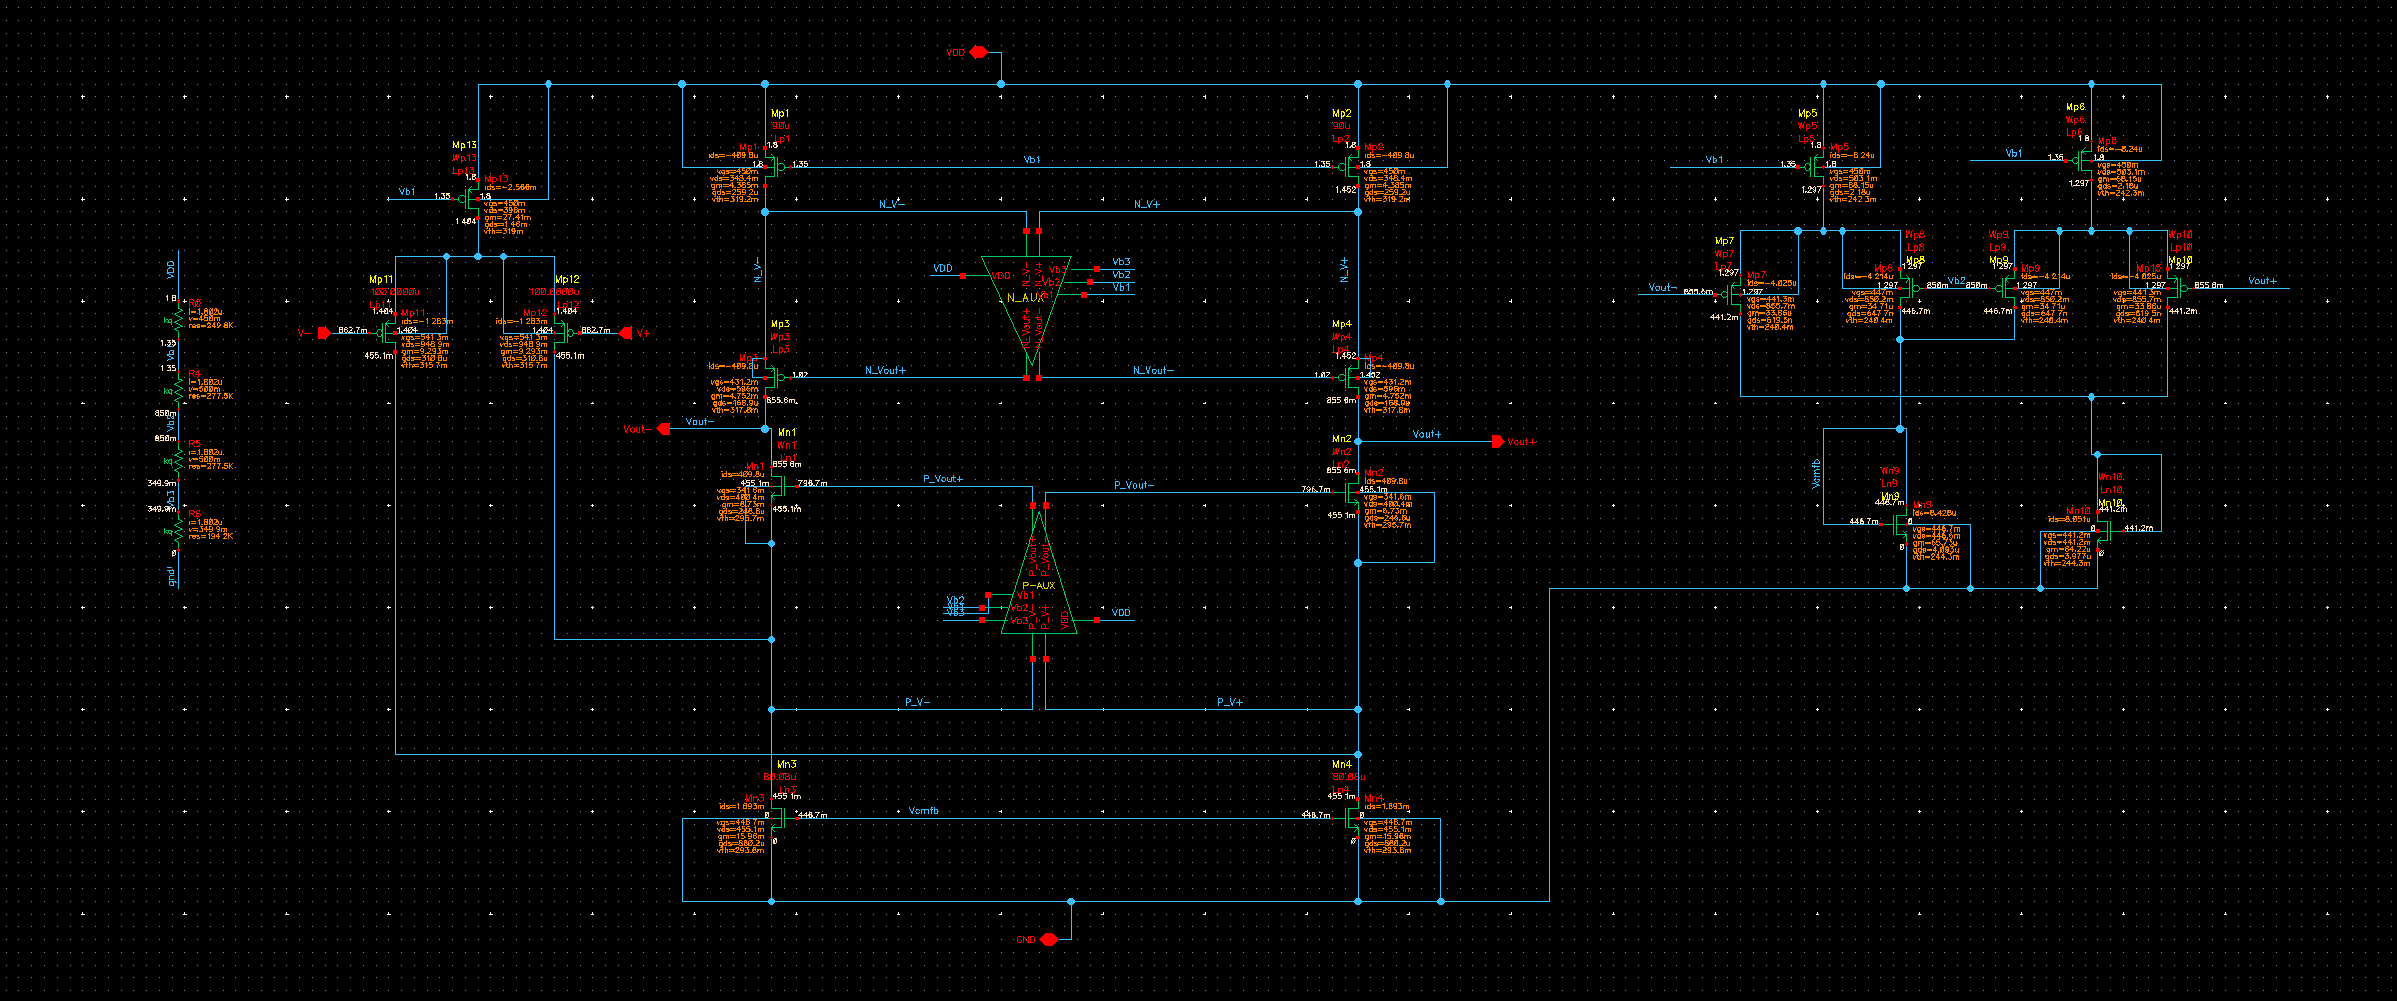
\includegraphics[width=\textwidth, height=0.8\textwidth]{main1_scematic.png}
    \caption{Schematic of the main amplifier circuit}
    \label{fig:main_circuit}
\end{figure}


The topology follows a folded cascode design, with each branch utilizing a gain booster of the same topology. For CMFB, an error amplifier is used, averaging the common-mode voltage at the input and responding to variations. 

\begin{figure}[H]
    \centering
    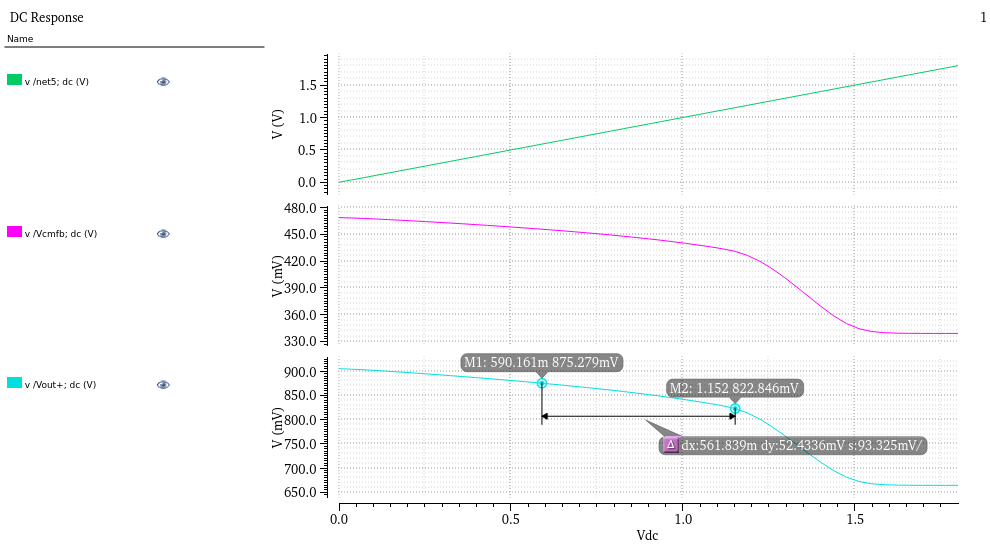
\includegraphics[width=0.7\textwidth]{CMFB_prove.png}
    \caption{CMFB Response: Output voltage stability and common-mode correction}
    \label{fig:cmfb_response}
\end{figure}

Figure \ref{fig:cmfb_response} illustrates how the output voltage remains stable within 50mV variation for a 0.5V operating range. Additionally, the CMFB circuit lowers the gate voltages of Mn3 and Mn4, reducing current in the branch and maintaining a fixed common-mode voltage.
\subsubsection{Biasing}
To provide the required voltages for the various circuit components, a simple resistor divider network was employed. The total resistance of the network sums to \textbf{1MΩ}, ensuring minimal power consumption while maintaining stable biasing. Additionally, all circuit components were designed to operate at the same bias voltages—\textbf{0.35V, 0.85V, and 1.35V}—to minimize the number of separate biasing circuits required within the system.

For the \textbf{DC input bias of the amplifier}, as discussed in the noise analysis section, we were unable to efficiently provide a stable \textbf{DC voltage} to the gates of the differential input pair without introducing excessive noise. To overcome this, we adopted the \textbf{self-biasing} technique exclusively for the input stage. This method allows the transistor to set its own gate voltage according to the flowing current. By isolating the source from the gate using an \textbf{input coupling capacitor}, the \textbf{gate effectively becomes floating} and naturally settles at an appropriate voltage.

Although this approach required fine-tuning of parameters to achieve the desired voltage, it proved to be highly effective and offers significant flexibility in circuit design.


\subsection{AC Analysis of Main Amplifier (Without Boosters)}
\begin{figure}[H]
    \centering
    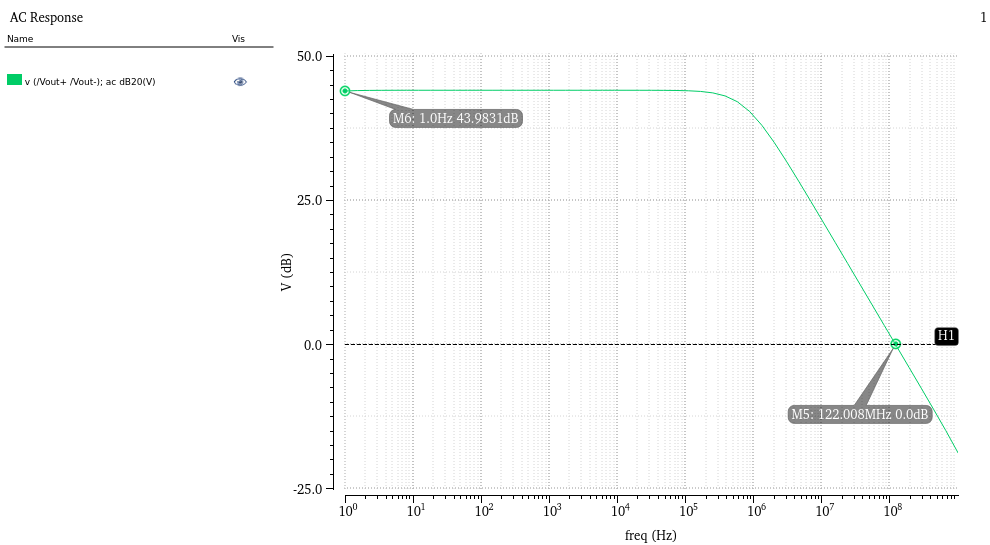
\includegraphics[width=0.7\textwidth]{AC_respose_MAIN_AMP_before.png}
    \caption{AC response of the main amplifier before adding gain boosters}
    \label{fig:ac_main_before}
\end{figure}

\begin{table}[h]
    \centering
    \begin{tabular}{ll}
        \toprule
        Parameter & Value \\
        \midrule
        Gain & 43.9 dB \\
        GBW & 122 MHz \\
        \bottomrule
    \end{tabular}
    \caption{AC performance of main amplifier (without boosters)}
    \label{tab:ac_main_before}
\end{table}

\subsection{Gain Boosting}
The gain boosting technique enhances the amplifier's DC gain by utilizing auxiliary amplifiers to increase the output impedance of the cascode transistors. In our design, two separate auxiliary amplifiers were implemented - one for the NMOS branch and one for the PMOS branch. These amplifiers create local feedback loops around their respective cascode transistors, actively regulating their gate voltages to maintain optimal operating points.

A critical aspect of our design was managing the bandwidth relationship between the main amplifier and the auxiliary amplifiers. To maintain stability, the gain-bandwidth product (GBW) of the auxiliary amplifiers was designed to be 2-3 times lower than the main amplifier's GBW. Initially, we aimed for a ratio of 2.5, achieving GBW values of 107.6 MHz and 74.9 MHz for the NMOS and PMOS boosters respectively, compared to the main amplifier's original GBW of 122 MHz.

The effectiveness of this approach is demonstrated by the significant improvement in output resistance, which increased from 110KΩ to 20MΩ after implementing the gain boosters. This resulted in a substantial enhancement of the overall DC gain from 43.9 dB to 95.8 dB, while maintaining stable operation with excellent phase margin. The success of this implementation validates our design choices in both the topology and sizing of the auxiliary amplifiers.


\subsection{Auxiliary Gain-Boosting Amplifiers}
The two auxiliary amplifiers were designed using a similar topology to the main amplifier, but different input transistors were selected to adapt to the required input voltage levels.

Additionally, for each booster, a smaller and weaker common-mode feedback (CMFB) circuit was designed using two transistors operating in the weak inversion (WI) region. This ensures proper common-mode regulation while maintaining minimal power consumption and avoiding interference with the main amplifier’s CMFB circuit.

\begin{figure}[h]
    \centering
    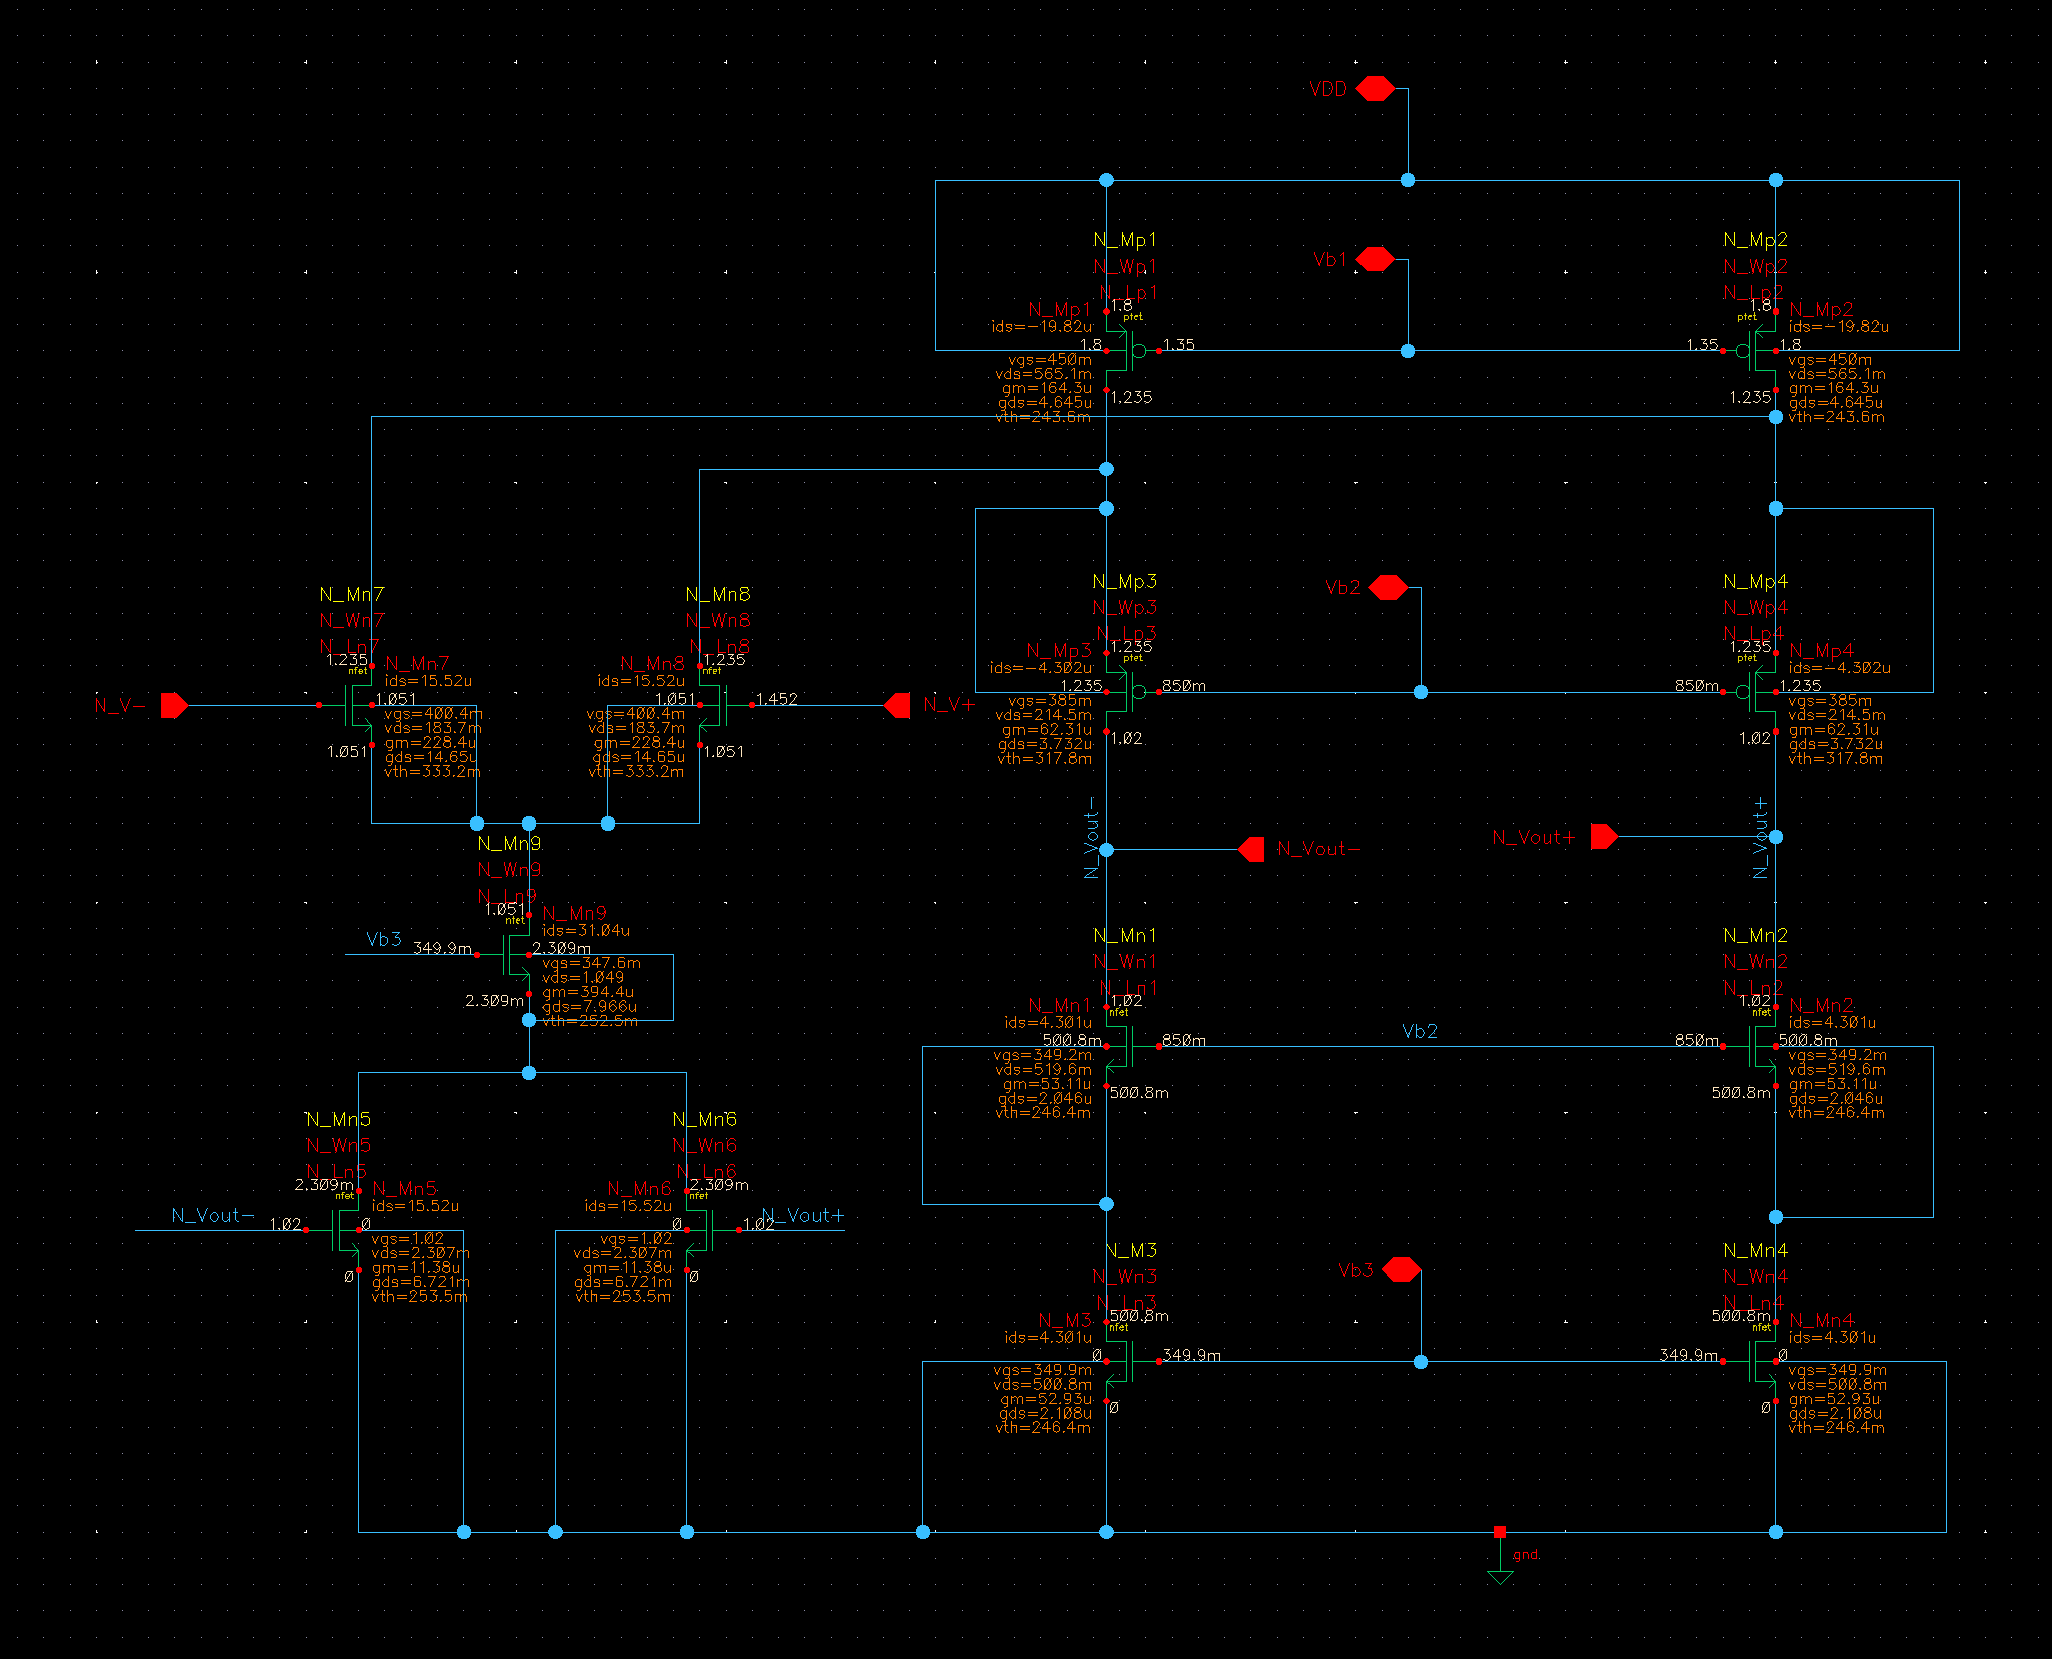
\includegraphics[width=0.7\textwidth]{N_AUX1_scematic.png}
    \caption{Schematic of the NMOS auxiliary gain booster}
    \label{fig:n_aux}
\end{figure}

\begin{figure}[h]
    \centering
    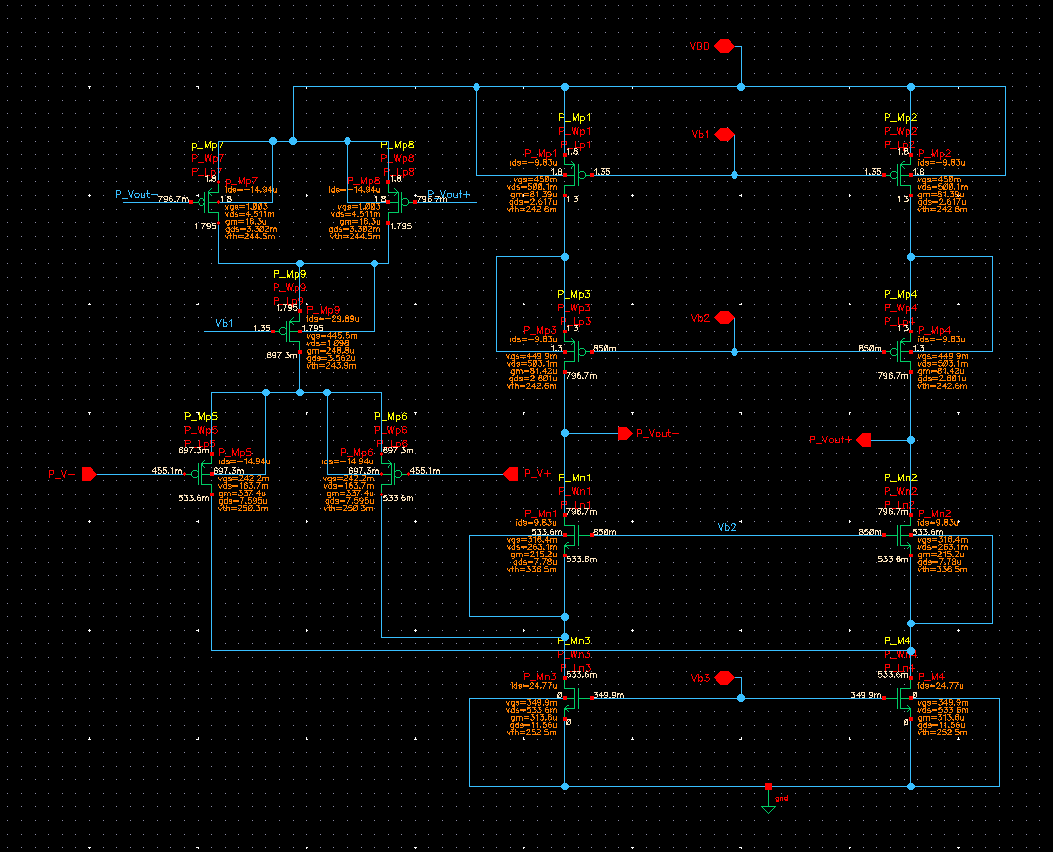
\includegraphics[width=0.7\textwidth]{P_AUX1_scematic.png}
    \caption{Schematic of the PMOS auxiliary gain booster}
    \label{fig:p_aux}
\end{figure}

The AC response of the auxiliary amplifiers was simulated while ensuring their outputs drive the main amplifier’s cascode nodes to match expected capacitive loads.

\begin{figure}[H]
    \centering
    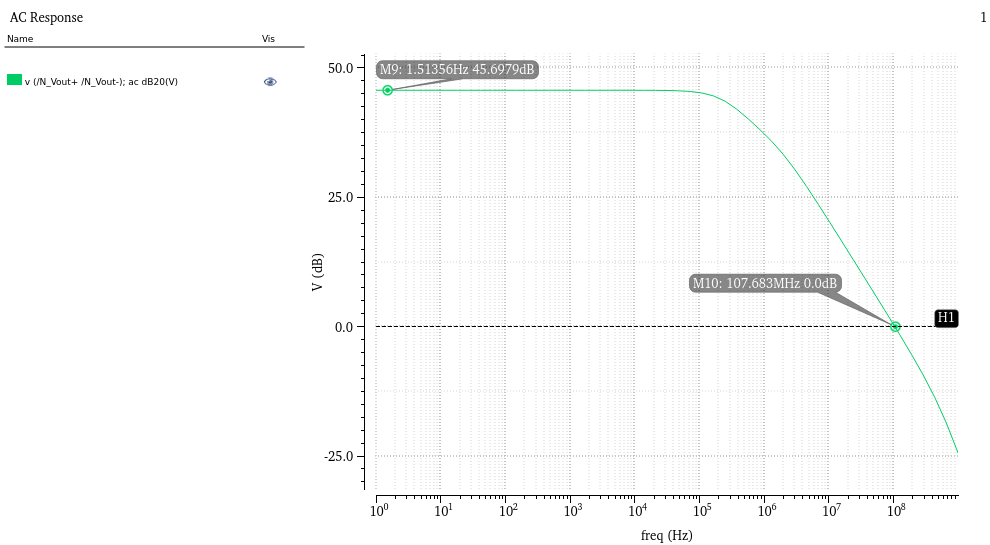
\includegraphics[width=0.7\textwidth]{AC_respose_N_AUX.png}
    \caption{AC response of NMOS auxiliary gain booster}
    \label{fig:ac_n_aux}
\end{figure}

\begin{figure}[H]
    \centering
    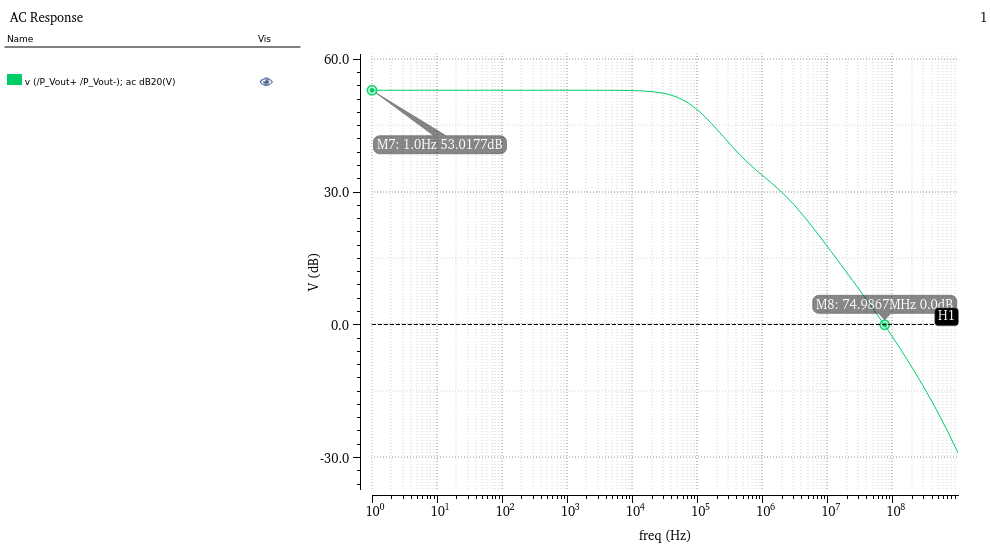
\includegraphics[width=0.7\textwidth]{AC_respose_P_AUX.png}
    \caption{AC response of PMOS auxiliary gain booster}
    \label{fig:ac_p_aux}
\end{figure}

\begin{table}[h]
    \centering
    \begin{tabular}{lll}
        \toprule
        Parameter & NMOS Booster & PMOS Booster \\
        \midrule
        Gain & 45.69 dB & 53 dB \\
        GBW & 107.6 MHz & 74.9 MHz \\
        \bottomrule
    \end{tabular}
    \caption{AC performance of auxiliary gain-boosting amplifiers}
    \label{tab:ac_aux}
\end{table}
\subsection{Post-Boosting AC Analysis}
After integrating the gain boosters, an additional AC analysis was performed on the main amplifier. The results are presented in Figure \ref{fig:ac_main_after}. It is evident that the boosters had a significant impact on the GBW, which decreased to 108.1 MHz, as a consequence of not maintaining the intended GBW ratio between the main amplifier and the auxiliary amplifiers. However, the drastic improvement in \textbf{gain}, which increased to \textbf{95.8 dB}, cannot be overlooked.

This substantial increase in gain is primarily attributed to a dramatic rise in output resistance. As illustrated in Figure \ref{fig:rout_comparison}, the output resistance increased from \textbf{110KΩ} to \textbf{20MΩ}, highlighting the effectiveness of the gain-boosting technique.

\begin{figure}[h]
    \centering
    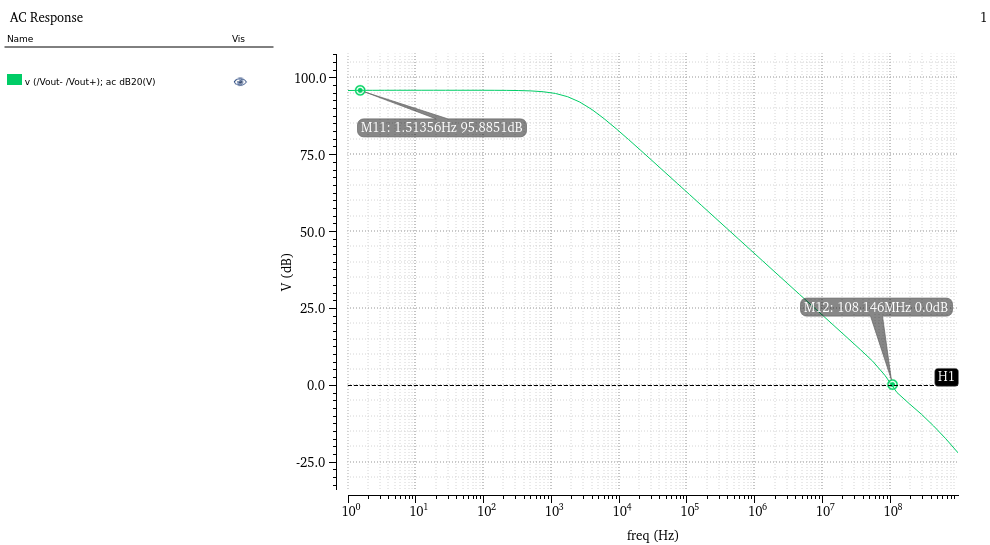
\includegraphics[width=0.7\textwidth]{AC_respose_MAIN_AMP_after.png}
    \caption{AC response of the main amplifier after gain boosting}
    \label{fig:ac_main_after}
\end{figure}

\begin{table}[H]
    \centering
    \begin{tabular}{ll}
        \toprule
        Parameter & Value \\
        \midrule
        Gain & 95.8 dB \\
        GBW & 108.1 MHz \\
        \bottomrule
    \end{tabular}
    \caption{AC performance of the main amplifier after gain boosting}
    \label{tab:ac_main_after}
\end{table}

\begin{figure}[H]
    \centering
    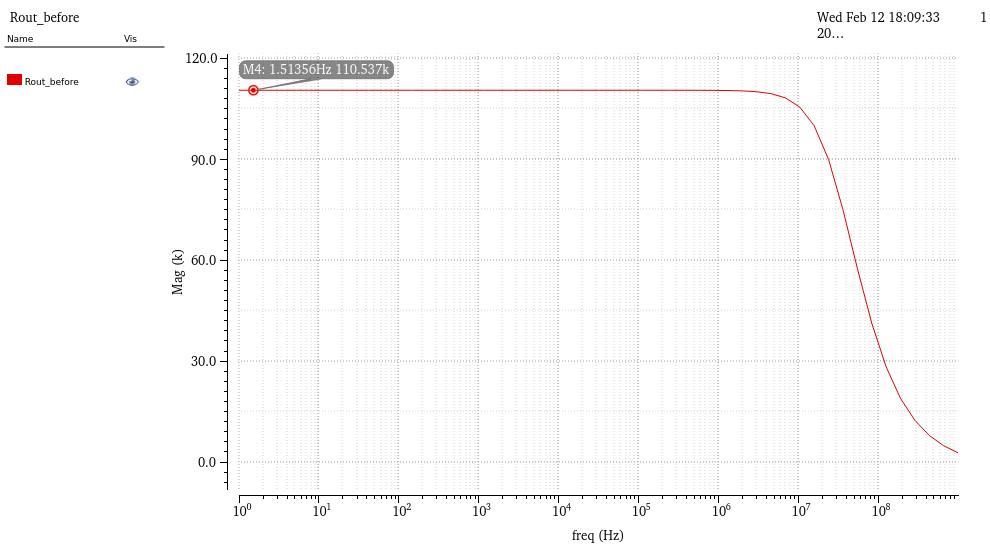
\includegraphics[width=0.48\textwidth]{Rout_befor.png}
    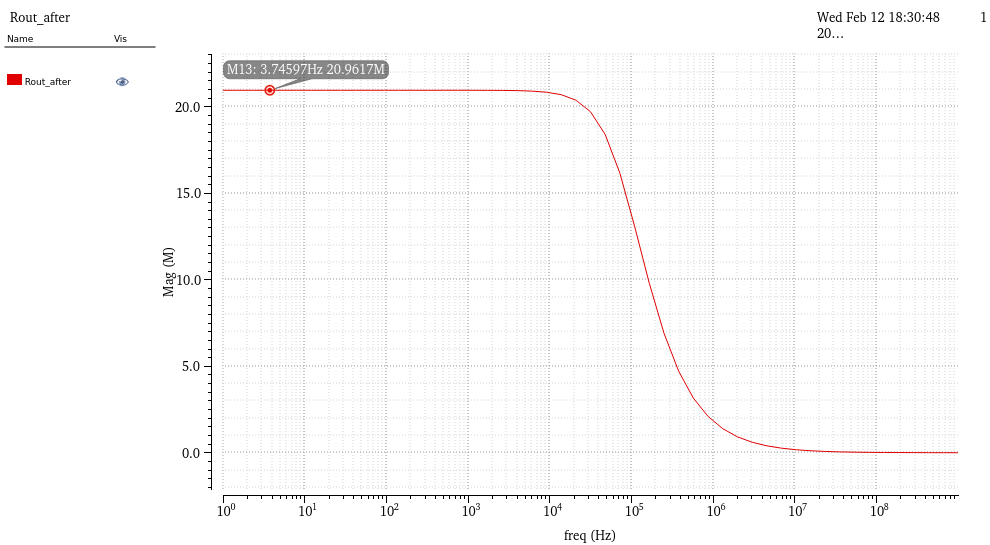
\includegraphics[width=0.48\textwidth]{Rout_after.png}
    \caption{Comparison of output resistance before and after gain boosting}
    \label{fig:rout_comparison}
\end{figure}

\pagebreak
\newpage

\subsection{Transistor Sizing Table}
The following table summarizes the transistor dimensions for the main amplifier and auxiliary circuits. The width-to-length (W/L) ratios are provided, with placeholders for transconductance ($g_m$) and output conductance ($g_{ds}$) values.

\begin{table}[h]
    \centering
    \begin{tabular}{|l|c|c|c|}
        \hline
        Transistor & W/L ($\mu m$) & $g_m$ (S) & $g_{ds}$ (S) \\
        \hline
        \multicolumn{4}{|c|}{\textbf{Main Amplifier}} \\
        \hline
        Mn1, Mn2 & 80.1/0.4 & 8.73m & 248.6u \\
        Mn3, Mn4 & 80.1/0.4 & 15.96m & 880.2u \\
        Mn9 & 0.7/1 & 66.73u & 4.09u \\
        Mn10 & 0.1/1 & 64.22u & 3.97u \\
        Mp1, Mp2 & 90/0.2 & 4.38m & 259.2u \\
        Mp3, Mp4 & 90/0.2 & 4.75m & 168.9u \\
        Mp11, Mp12 & 100/0.2 & 9.29m & 310.8u \\
        Mp13 & 500/0.2 & 27.41m & 1.46m \\
        \hline
        \multicolumn{4}{|c|}{\textbf{N-BOOSTER}} \\
        \hline
        Mn1, Mn2 & 0.9/1 & 53.1u & 2.8u \\
        Mn3, Mn4 & 0.9/1 & 32.9u & 2.1u \\
        Mn5, Mn6 & 20/1 & 11.39u & 8.72m \\
        Mn7, Mn8 & 1.8/0.2 & 228.4u & 14.85u \\
        Mn9 & 5.4/1 & 394u & 7.9u \\
        Mp1, Mp2 & 11.1/1 & 164.3u & 4.6u \\
        Mp3, Mp4 & 2.4/0.2 & 62.3u & 3.73u \\
        \hline
        \multicolumn{4}{|c|}{\textbf{P-BOOSTER}} \\
        \hline
        Mn1, Mn2 & 5/0.2 & 215.2u & 7.7u \\
        Mn3, Mn4 & 5/1 & 313.6u & 11.56u \\
        Mp1, Mp2 & 5.7/1 & 81.39u & 2.6u \\
        Mp3, Mp4 & 5.17/1 & 81.42u & 2.6u \\
        Mp5, Mp6 & 150/0.8 & 337.4u & 7.59u \\
        Mp7, Mp8 & 53.6/1 & 16.3u & 3.3m \\
        Mp9 & 15.8/1 & 248.8u & 3.56u \\
        \hline
    \end{tabular}
    \caption{Transistor sizing, transconductance ($g_m$), and output conductance ($g_{ds}$)}
    \label{tab:transistor_specs}
\end{table}

\subsection{Power Consumption}
The total current consumption of the circuit is measured at \textbf{3.493mA}, with a supply voltage of \textbf{1.8V}. This results in a total power consumption of:
\begin{equation}
P = V_{DD} \times I_{total} = 1.8V \times 3.493mA = 6.287mW
\end{equation}
This power level is within the design constraints, ensuring both efficiency and high performance.

\begin{figure}[H]
\centering
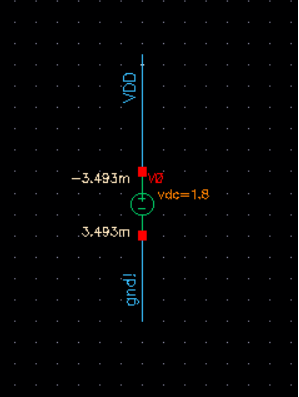
\includegraphics[width=0.4\textwidth]{power.png}
\caption{Power Consumption Analysis}
\label{fig:power}
\end{figure}
\newpage
\section{AC Analysis}
\subsection{Common-Mode Rejection Ratio (CMRR)}
The common-mode rejection ratio (CMRR) is a critical parameter in differential amplifiers, measuring the ability to suppress common-mode signals. Figure \ref{fig:cmrr} presents the simulated CMRR response.

\begin{figure}[H]
\centering
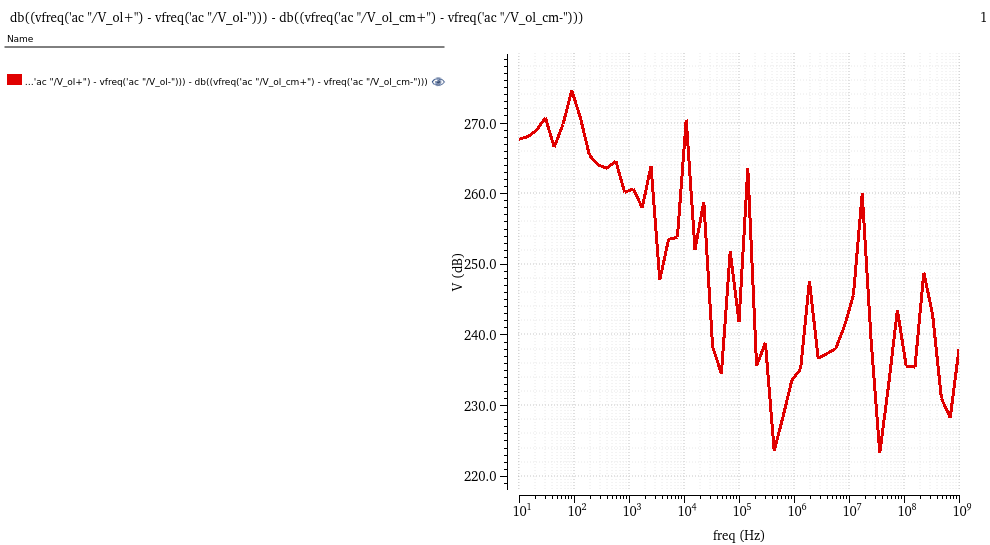
\includegraphics[width=0.5\textwidth]{CMRR.png}
\caption{CMRR Response of the Amplifier}
\label{fig:cmrr}
\end{figure}

The average CMRR value is approximately \textbf{250 dB}, indicating excellent common-mode rejection performance. This ensures that unwanted noise and common-mode disturbances have minimal impact on the differential signal.

\subsection{Slew Rate (SR)}
The slew rate (SR) represents the maximum rate of change of the output voltage and is a key parameter in determining the amplifier's ability to handle fast transient signals. The measured slew rate is extracted manually from the transient response shown in Figure \ref{fig:sr}.

\begin{figure}[H]
\centering
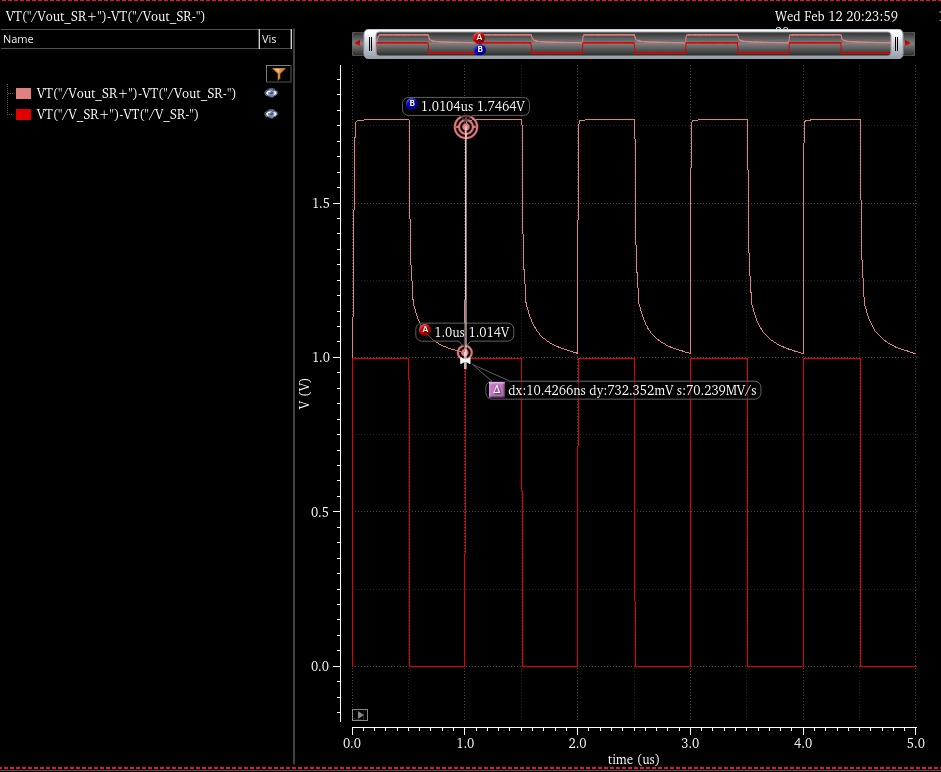
\includegraphics[width=0.4\textwidth]{SR.png}
\caption{Measured Slew Rate of the Amplifier}
\label{fig:sr}
\end{figure}

The measured slew rate is \textbf{70 V/$\mu$s}. This is an important parameter as it directly affects the settling time of the amplifier and determines whether the design meets the required transient performance specifications.
\newpage
\section{Noise Analysis}

\subsection{Design Challenges and Solutions}

We acknowledge that we did not conduct thorough noise parameter testing during the initial design phase. Consequently, upon finalizing the amplifier, we achieved an extremely powerful and fast design—but with excessive noise! Meeting the noise specification turned out to be the most challenging requirement.



Our noise reduction strategy involved several key innovations:

\begin{itemize}
\item \textbf{Feedback Network Optimization:}
\begin{itemize}
\item Implementation of a parallel RC network ($R_f = 500M\Omega$, $C_f = 20pF$)
\item Addition of source capacitance ($C_s = 60pF$)
\item The resistor drastically reduced the overall noise level by attenuating low-frequency gain in the closed-loop system, effectively suppressing the dominant $1/f$ noise.
\end{itemize}
\item \textbf{Transistor Layout Optimization:}
\begin{itemize}
\item Splitting transistors into multiple fingers proved highly effective in reducing noise, particularly gate resistance noise, which was significantly mitigated using this approach.
\end{itemize}
\end{itemize}

Figure \ref{fig:feedback_net} illustrates the proposed feedback network used to mitigate noise.

\begin{figure}[H]
\centering
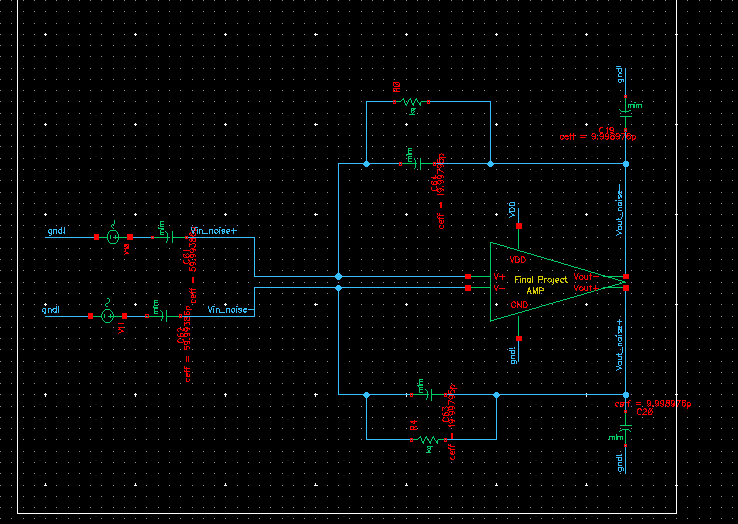
\includegraphics[width=0.7\textwidth]{feedback_net.png}
\caption{Proposed Feedback Network for Noise Reduction}
\label{fig:feedback_net}
\end{figure}

The resulting integrated noise floor of $18 nV/\sqrt{Hz}$  represents the optimal compromise between noise performance and maintaining the amplifier's high-speed capabilities. As shown in Figure \ref{fig:noise_summary}, this configuration effectively addresses both thermal and $1/f$ noise components.

\begin{figure}[H]
\centering
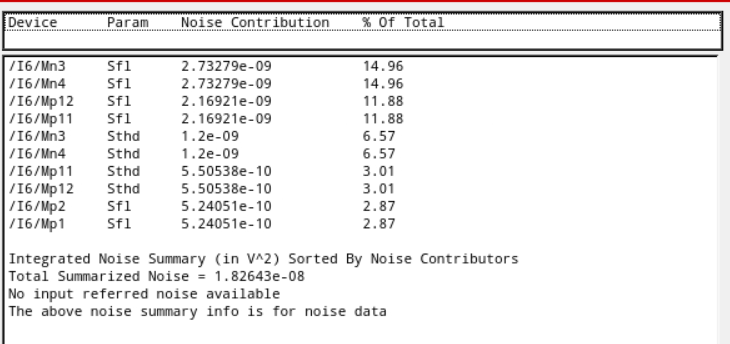
\includegraphics[width=0.7\textwidth]{noise_summary.png}
\caption{Final Noise Summary of the Amplifier}
\label{fig:noise_summary}
\end{figure}

Further reductions in noise were difficult to achieve without significantly compromising the amplifier's overall performance, demonstrating the fundamental trade-off between noise optimization and maintaining high-speed operation.


\subsection{Dynamic Range (DR) Estimation}

To determine the dynamic range, we performed a sweep on increasing amplitude values and identified that the maximum differential output voltage, where the waveform remains sinusoidal, is \textbf{0.48V}. This results in a peak output voltage of \textbf{1.35V}.

To confirm this, we analyzed the Total Harmonic Distortion (THD) of the Discrete Fourier Transform (DFT) of the output signal. The measured THD was found to be \textbf{-34 dB}, which is still within the acceptable range for a sinusoidal waveform.

\begin{figure}[H]
\centering
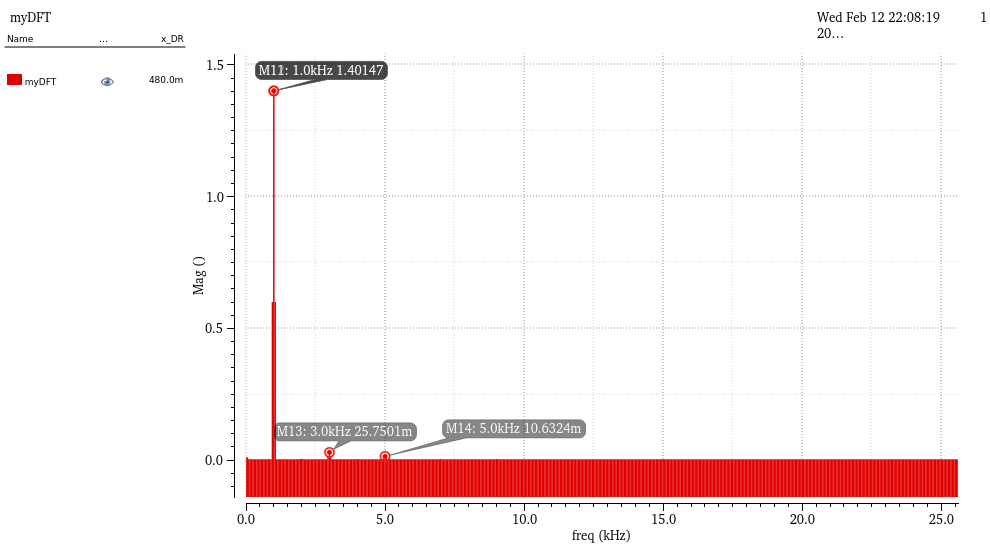
\includegraphics[width=0.7\textwidth]{DR.png}
\caption{Dynamic Range Measurement Results}
\label{fig:dr}
\end{figure}

\begin{figure}[H]
\centering
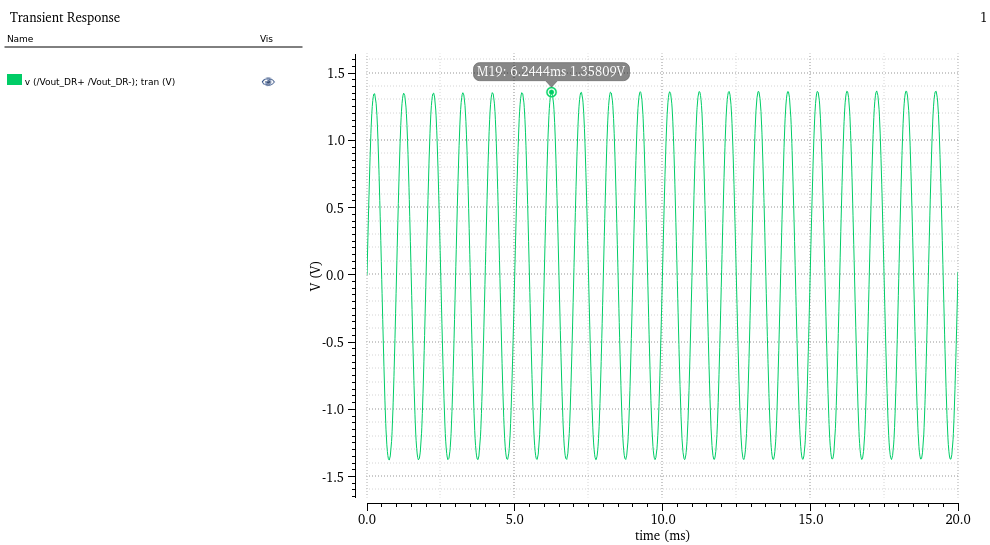
\includegraphics[width=0.7\textwidth]{sine_for_DR.png}
\caption{Sinusoidal Signal at Maximum Dynamic Range}
\label{fig:sine_dr}
\end{figure}

Using the given definition of dynamic range:
\begin{equation}
DR = 10 \log_{10} \left( \frac{P_{\text{peak}}}{P_{\text{noise}}} \right)
\end{equation}

Substituting the values:
\begin{equation}
DR = 10 \log_{10} \left( \frac{(1.35V)^2}{18nV} \right) = 80.05 \text{ dB}
\end{equation}

Thus, the calculated \textbf{Dynamic Range (DR)} is \textbf{80.05 dB}. Further noise reduction could marginally improve DR, but this value already meets the required specifications without degrading the amplifier’s performance.
\section{Stability Analysis}

\subsection{Phase Margin and Stability Considerations}
The stability analysis of our amplifier demonstrates exceptional performance, particularly in terms of phase margin and closed-loop behavior. Our measurements yielded several key results:

\begin{itemize}
    \item \textbf{Closed-Loop Performance:}
    \begin{itemize}
        \item Achieved precise gain of 3 V/V as specified
        \item Bandwidth optimization through careful feedback network design
        \item Excellent linearity across the operating range
    \end{itemize}
    
    \item \textbf{Phase Margin Analysis:}
    \begin{itemize}
        \item Measured phase margin of 88° at unity gain frequency of 14 MHz
        \item This substantial margin ensures:
        \begin{itemize}
            \item Zero overshoot in step response
            \item Robust stability across process variations
            \item Reliable operation under varying load conditions
        \end{itemize}
    \end{itemize}
    
    \item \textbf{Stability Enhancement Techniques:}
    \begin{itemize}
        \item Strategic placement of poles through gain-booster design
        \item Careful consideration of feedback network components
        \item Optimization of compensation scheme without requiring additional capacitors
    \end{itemize}
\end{itemize}

The notably high phase margin of 88° represents a significant achievement, far exceeding the minimum requirement of 60°. This margin provides substantial immunity to process variations and ensures consistent performance across different operating conditions.

\begin{figure}[H]
    \centering
    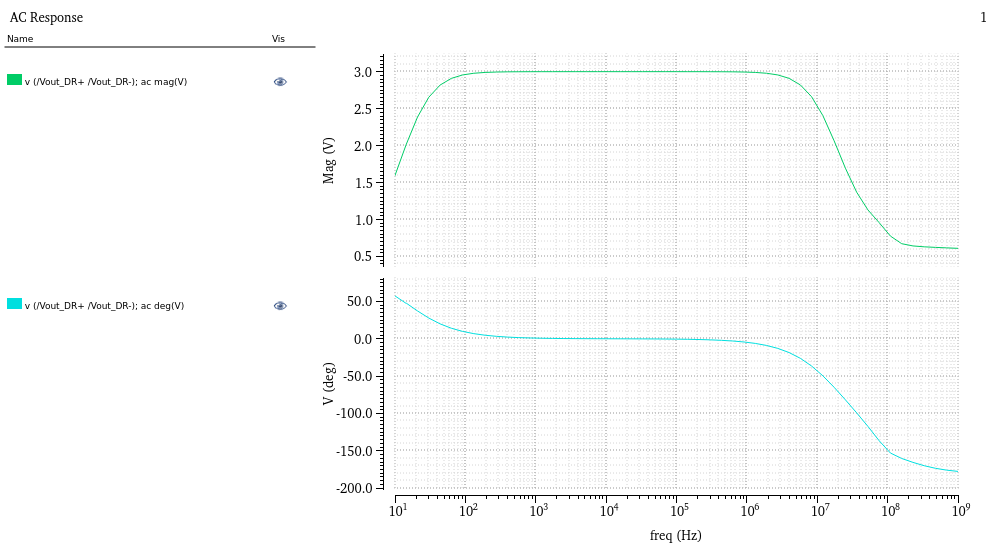
\includegraphics[width=0.7\textwidth]{close_loop_gain.png}
    \caption{Measured Closed-Loop Gain and phase of the Amplifier}
    \label{fig:close_loop_gain}
\end{figure}

\begin{figure}[H]
    \centering
    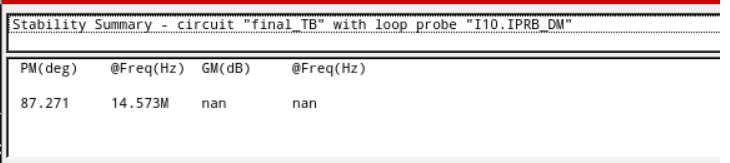
\includegraphics[width=0.7\textwidth]{std_summary.png}
    \caption{Stability Summary of the Amplifier}
    \label{fig:stability_summary}
\end{figure}

Since the amplifier gain does not reach \textbf{180°}, there is no defined gain margin (GM) for this design.

\subsection{Step Response and Settling Behavior}
The amplifier's excellent stability is further validated by its step response characteristics:

\begin{itemize}
    \item Settling time of 41 ns for a 0.3V differential step
    \item Clean settling behavior with minimal ringing
    \item Final settling error well within the 0.5 mV specification
\end{itemize}

These results confirm the successful implementation of our stability optimization strategy, demonstrating that the design achieves both high performance and robust stability.

\begin{figure}[H]
    \centering
    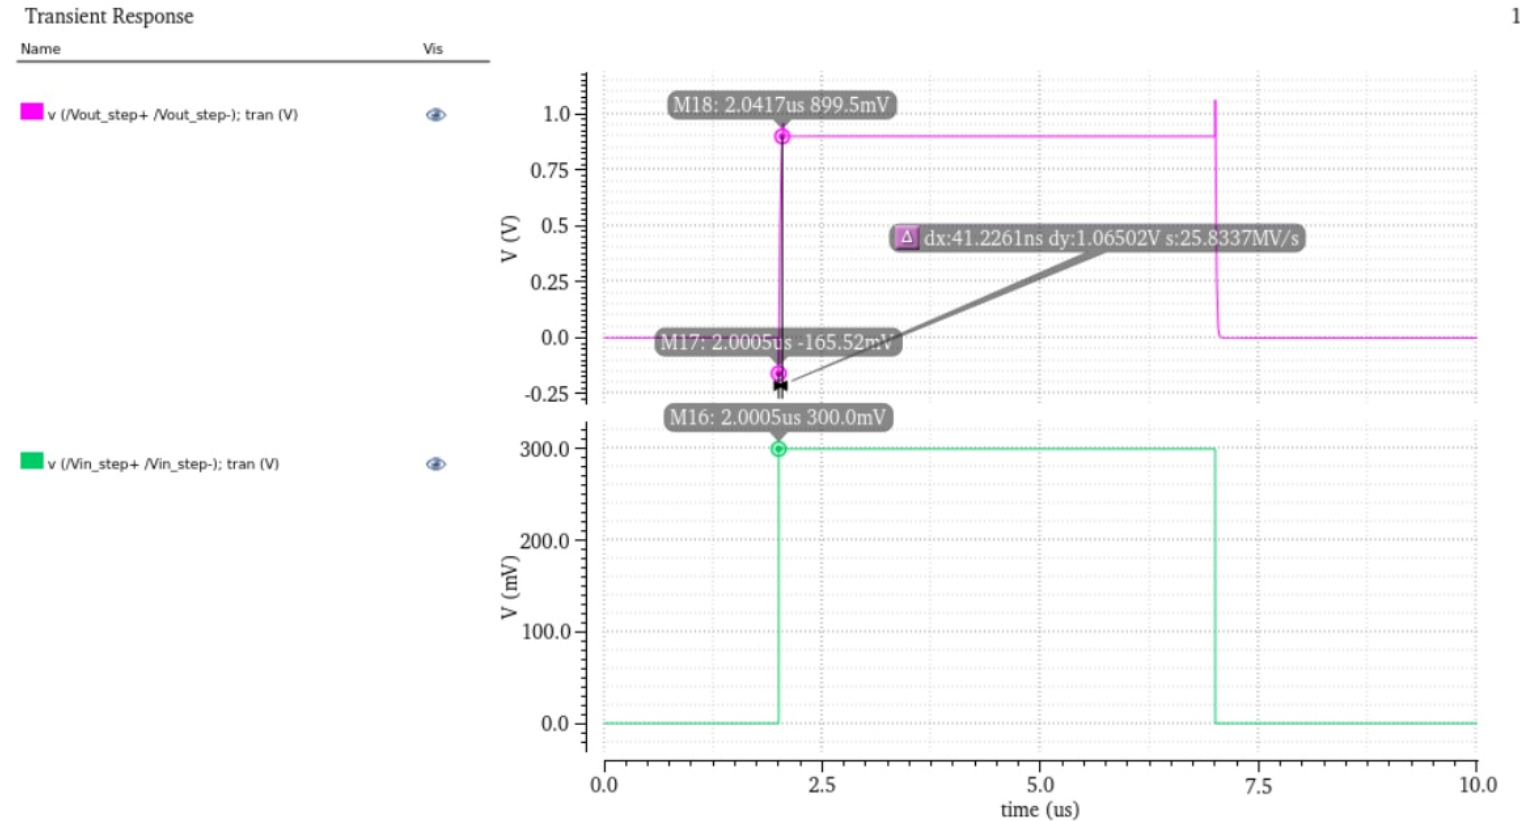
\includegraphics[width=0.7\textwidth]{settling_time.png}
    \caption{Measured Settling Time of the Amplifier}
    \label{fig:settling_time}
\end{figure}


\section{Conclusion}
This report presents the design and analysis of a fully differential amplifier using a folded cascode topology with gain boosting. Through careful design optimizations, we successfully achieved high gain, stability, and noise reduction while maintaining low power consumption. The amplifier met all key specifications, demonstrating excellent phase margin, dynamic range, and settling performance.

\section{Performance Summary}
\begin{table}[H]
    \centering
    \begin{tabular}{|l|c|c|}
        \hline
        Specification & Required & Achieved \\
        \hline
        Closed-Loop Gain & 3 & 3 \\
        Phase Margin (PM) & > 60° & 88° \\
        Dynamic Range (DR) & > 80 dB & 80.05 dB \\
        Settling Time & < 50 ns & 41 ns \\
        Settling Error & < 0.5 mV & 482.8 µV \\
        Power Consumption & As low as possible & 6.287 mW \\
        \hline
    \end{tabular}
    \caption{Performance Summary: Required vs. Achieved}
    \label{tab:performance_summary}
\end{table}

\section{References and Acknowledgments}
We found the following research articles particularly useful in guiding our design and implementation process:

\begin{itemize}
\item \textit{Design of a 2 mW Power 112 dB Gain-Boosted Folded Cascode Amplifier in 0.18µm Process}, available at \url{https://www.researchgate.net/publication/355835467_Design_of_a_2_mW_Power_112_dB_Gain-Boosted_Folded_Cascode_Amplifier_in_018m_Process}. This paper was especially influential as we adopted the topology implemented in this work.
\item \textit{A 252W Wide-Swing Fully Differential Two-Stage CMOS OTA for Low-Power Applications in NCSU 0.18µm PDK}, available at \url{https://www.researchgate.net/publication/353247569_A_252W_Wide-Swing_Fully_Differential_Two-Stage_CMOS_OTA_for_Low-Power_Applications_in_NCSU_018m_PDK}.
\item \textit{Fully-Differential Opamp Design}, available at \url{https://www.researchgate.net/publication/327546297_Fully-differential_opamp_design}.
\end{itemize}


\end{document}
